\documentclass[twoside]{book}

% Packages required by doxygen
\usepackage{calc}
\usepackage{doxygen}
\usepackage{graphicx}
\usepackage[utf8]{inputenc}
\usepackage{makeidx}
\usepackage{multicol}
\usepackage{multirow}
\usepackage{textcomp}
\usepackage[table]{xcolor}

% Font selection
\usepackage[T1]{fontenc}
\usepackage{mathptmx}
\usepackage[scaled=.90]{helvet}
\usepackage{courier}
\usepackage{amssymb}
\usepackage{sectsty}
\renewcommand{\familydefault}{\sfdefault}
\allsectionsfont{%
  \fontseries{bc}\selectfont%
  \color{darkgray}%
}
\renewcommand{\DoxyLabelFont}{%
  \fontseries{bc}\selectfont%
  \color{darkgray}%
}

% Page & text layout
\usepackage{geometry}
\geometry{%
  a4paper,%
  top=2.5cm,%
  bottom=2.5cm,%
  left=2.5cm,%
  right=2.5cm%
}
\tolerance=750
\hfuzz=15pt
\hbadness=750
\setlength{\emergencystretch}{15pt}
\setlength{\parindent}{0cm}
\setlength{\parskip}{0.2cm}
\makeatletter
\renewcommand{\paragraph}{%
  \@startsection{paragraph}{4}{0ex}{-1.0ex}{1.0ex}{%
    \normalfont\normalsize\bfseries\SS@parafont%
  }%
}
\renewcommand{\subparagraph}{%
  \@startsection{subparagraph}{5}{0ex}{-1.0ex}{1.0ex}{%
    \normalfont\normalsize\bfseries\SS@subparafont%
  }%
}
\makeatother

% Headers & footers
\usepackage{fancyhdr}
\pagestyle{fancyplain}
\fancyhead[LE]{\fancyplain{}{\bfseries\thepage}}
\fancyhead[CE]{\fancyplain{}{}}
\fancyhead[RE]{\fancyplain{}{\bfseries\leftmark}}
\fancyhead[LO]{\fancyplain{}{\bfseries\rightmark}}
\fancyhead[CO]{\fancyplain{}{}}
\fancyhead[RO]{\fancyplain{}{\bfseries\thepage}}
\fancyfoot[LE]{\fancyplain{}{}}
\fancyfoot[CE]{\fancyplain{}{}}
\fancyfoot[RE]{\fancyplain{}{\bfseries\scriptsize Generated on Sat Dec 7 2013 17\-:08\-:34 for Q\-Music Generator by Doxygen }}
\fancyfoot[LO]{\fancyplain{}{\bfseries\scriptsize Generated on Sat Dec 7 2013 17\-:08\-:34 for Q\-Music Generator by Doxygen }}
\fancyfoot[CO]{\fancyplain{}{}}
\fancyfoot[RO]{\fancyplain{}{}}
\renewcommand{\footrulewidth}{0.4pt}
\renewcommand{\chaptermark}[1]{%
  \markboth{#1}{}%
}
\renewcommand{\sectionmark}[1]{%
  \markright{\thesection\ #1}%
}

% Indices & bibliography
\usepackage{natbib}
\usepackage[titles]{tocloft}
\setcounter{tocdepth}{3}
\setcounter{secnumdepth}{5}
\makeindex

% Hyperlinks (required, but should be loaded last)
\usepackage{ifpdf}
\ifpdf
  \usepackage[pdftex,pagebackref=true]{hyperref}
\else
  \usepackage[ps2pdf,pagebackref=true]{hyperref}
\fi
\hypersetup{%
  colorlinks=true,%
  linkcolor=blue,%
  citecolor=blue,%
  unicode%
}

% Custom commands
\newcommand{\clearemptydoublepage}{%
  \newpage{\pagestyle{empty}\cleardoublepage}%
}


%===== C O N T E N T S =====

\begin{document}

% Titlepage & ToC
\hypersetup{pageanchor=false}
\pagenumbering{roman}
\begin{titlepage}
\vspace*{7cm}
\begin{center}%
{\Large Q\-Music Generator \\[1ex]\large 1.\-0 }\\
\vspace*{1cm}
{\large Generated by Doxygen 1.8.5}\\
\vspace*{0.5cm}
{\small Sat Dec 7 2013 17:08:34}\\
\end{center}
\end{titlepage}
\clearemptydoublepage
\tableofcontents
\clearemptydoublepage
\pagenumbering{arabic}
\hypersetup{pageanchor=true}

%--- Begin generated contents ---
\chapter{applicationmusic}
\label{md_applicationmusic__r_e_a_d_m_e}
\hypertarget{md_applicationmusic__r_e_a_d_m_e}{}
\input{md_applicationmusic__r_e_a_d_m_e}
\chapter{Hierarchical Index}
\section{Class Hierarchy}
This inheritance list is sorted roughly, but not completely, alphabetically\-:\begin{DoxyCompactList}
\item \contentsline{section}{Chord}{\pageref{class_chord}}{}
\item \contentsline{section}{Not\-Connected}{\pageref{class_not_connected}}{}
\item \contentsline{section}{Note}{\pageref{class_note}}{}
\item \contentsline{section}{Partition}{\pageref{class_partition}}{}
\item Q\-Exception\begin{DoxyCompactList}
\item \contentsline{section}{Not\-J\-S\-O\-N\-Exception}{\pageref{class_not_j_s_o_n_exception}}{}
\end{DoxyCompactList}
\item Q\-Main\-Window\begin{DoxyCompactList}
\item \contentsline{section}{no\-Skin}{\pageref{classno_skin}}{}
\end{DoxyCompactList}
\end{DoxyCompactList}

\chapter{Class Index}
\section{Class List}
Here are the classes, structs, unions and interfaces with brief descriptions\-:\begin{DoxyCompactList}
\item\contentsline{section}{\hyperlink{class_chord}{Chord} }{\pageref{class_chord}}{}
\item\contentsline{section}{\hyperlink{classno_skin}{no\-Skin} \\*This class is used to represent all windows, no matter its layout }{\pageref{classno_skin}}{}
\item\contentsline{section}{\hyperlink{class_not_connected}{Not\-Connected} }{\pageref{class_not_connected}}{}
\item\contentsline{section}{\hyperlink{class_note}{Note} }{\pageref{class_note}}{}
\item\contentsline{section}{\hyperlink{class_not_j_s_o_n_exception}{Not\-J\-S\-O\-N\-Exception} }{\pageref{class_not_j_s_o_n_exception}}{}
\item\contentsline{section}{\hyperlink{class_partition}{Partition} }{\pageref{class_partition}}{}
\end{DoxyCompactList}

\chapter{Class Documentation}
\hypertarget{class_chord}{\section{Chord Class Reference}
\label{class_chord}\index{Chord@{Chord}}
}
\subsection*{Public Member Functions}
\begin{DoxyCompactItemize}
\item 
\hypertarget{class_chord_af662a96e956354ec9c37980546bcd133}{{\bfseries Chord} (std\-::vector$<$ \hyperlink{class_note}{Note} $>$ notes, double duration, double volume)}\label{class_chord_af662a96e956354ec9c37980546bcd133}

\item 
\hypertarget{class_chord_a1354afa1c0651647de48e47a2c9575f6}{double {\bfseries get\-Duration} () const }\label{class_chord_a1354afa1c0651647de48e47a2c9575f6}

\item 
\hypertarget{class_chord_a375d61538651858dd78698d62de2901b}{void {\bfseries set\-Duration} (double duration)}\label{class_chord_a375d61538651858dd78698d62de2901b}

\item 
\hypertarget{class_chord_a6aa66a8c71c77105119d81010a018bc5}{double {\bfseries get\-Volume} () const }\label{class_chord_a6aa66a8c71c77105119d81010a018bc5}

\item 
\hypertarget{class_chord_a2a7fbd2d39c0e2180123cb1edadf4b25}{void {\bfseries set\-Volume} (double volume)}\label{class_chord_a2a7fbd2d39c0e2180123cb1edadf4b25}

\item 
\hypertarget{class_chord_af003cd409e691665f4f366151bb6a288}{void {\bfseries play} ()}\label{class_chord_af003cd409e691665f4f366151bb6a288}

\end{DoxyCompactItemize}


The documentation for this class was generated from the following files\-:\begin{DoxyCompactItemize}
\item 
applicationmusic/model/chord.\-h\item 
applicationmusic/model/chord.\-cpp\end{DoxyCompactItemize}

\hypertarget{classno_skin}{\section{no\-Skin Class Reference}
\label{classno_skin}\index{no\-Skin@{no\-Skin}}
}


The documentation for this class was generated from the following files\-:\begin{DoxyCompactItemize}
\item 
applicationmusic/graphic/noskin.\-h\item 
applicationmusic/graphic/noskin.\-cpp\end{DoxyCompactItemize}

\hypertarget{class_not_connected}{\section{Not\-Connected Class Reference}
\label{class_not_connected}\index{Not\-Connected@{Not\-Connected}}
}
\subsection*{Public Member Functions}
\begin{DoxyCompactItemize}
\item 
virtual const char $\ast$ \hyperlink{class_not_connected_a3f5dbfd48407c041dee2d89169dd5b98}{what} () const   throw ()
\begin{DoxyCompactList}\small\item\em Describes the type of the error. Message might be shown to the user. \end{DoxyCompactList}\end{DoxyCompactItemize}


\subsection{Member Function Documentation}
\hypertarget{class_not_connected_a3f5dbfd48407c041dee2d89169dd5b98}{\index{Not\-Connected@{Not\-Connected}!what@{what}}
\index{what@{what}!NotConnected@{Not\-Connected}}
\subsubsection[{what}]{\setlength{\rightskip}{0pt plus 5cm}virtual const char$\ast$ Not\-Connected\-::what (
\begin{DoxyParamCaption}
{}
\end{DoxyParamCaption}
) const throw  ) \hspace{0.3cm}{\ttfamily [virtual]}}}\label{class_not_connected_a3f5dbfd48407c041dee2d89169dd5b98}


Describes the type of the error. Message might be shown to the user. 

\begin{DoxyReturn}{Returns}
A string describing the error 
\end{DoxyReturn}


The documentation for this class was generated from the following files\-:\begin{DoxyCompactItemize}
\item 
applicationmusic/graphic/notconnected.\-h\item 
applicationmusic/graphic/notconnected.\-cpp\end{DoxyCompactItemize}

\hypertarget{class_note}{\section{Note Class Reference}
\label{class_note}\index{Note@{Note}}
}
\subsection*{Public Member Functions}
\begin{DoxyCompactItemize}
\item 
\hypertarget{class_note_ad7dcafc723e68569639bd58bba6da623}{{\bfseries Note} (std\-::string name, int frequency)}\label{class_note_ad7dcafc723e68569639bd58bba6da623}

\item 
\hypertarget{class_note_acfef52222dab8bb2e15610643aa6c2ec}{void {\bfseries set\-Name} (std\-::string name)}\label{class_note_acfef52222dab8bb2e15610643aa6c2ec}

\item 
\hypertarget{class_note_a6be428300ec726fcab134b0d0e388401}{std\-::string {\bfseries get\-Name} () const }\label{class_note_a6be428300ec726fcab134b0d0e388401}

\item 
\hypertarget{class_note_abe02bd4d9f5a40e0f1222dd4e3c89875}{void {\bfseries set\-Frequency} (int frequency)}\label{class_note_abe02bd4d9f5a40e0f1222dd4e3c89875}

\item 
\hypertarget{class_note_a07d9c28685d79137e8a4073a0247dae5}{int {\bfseries get\-Frequency} () const }\label{class_note_a07d9c28685d79137e8a4073a0247dae5}

\item 
\hypertarget{class_note_a2eb9c1687f4849e78119d51d5966bf78}{void {\bfseries play} (double volume)}\label{class_note_a2eb9c1687f4849e78119d51d5966bf78}

\end{DoxyCompactItemize}


The documentation for this class was generated from the following files\-:\begin{DoxyCompactItemize}
\item 
applicationmusic/model/note.\-h\item 
applicationmusic/model/note.\-cpp\end{DoxyCompactItemize}

\hypertarget{class_not_j_s_o_n_exception}{\section{Not\-J\-S\-O\-N\-Exception Class Reference}
\label{class_not_j_s_o_n_exception}\index{Not\-J\-S\-O\-N\-Exception@{Not\-J\-S\-O\-N\-Exception}}
}
Inheritance diagram for Not\-J\-S\-O\-N\-Exception\-:\begin{figure}[H]
\begin{center}
\leavevmode
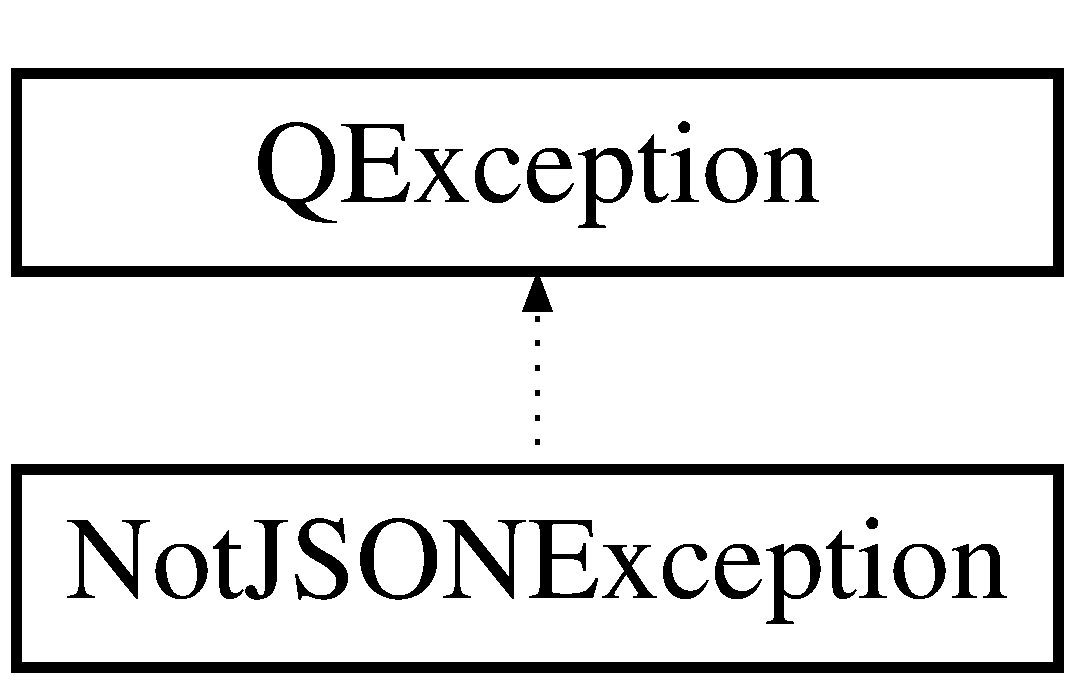
\includegraphics[height=2.000000cm]{class_not_j_s_o_n_exception}
\end{center}
\end{figure}
\subsection*{Public Member Functions}
\begin{DoxyCompactItemize}
\item 
virtual const char $\ast$ \hyperlink{class_not_j_s_o_n_exception_a4578c6ead67651a6b7f7ef46fc6ca579}{what} () const   throw ()
\begin{DoxyCompactList}\small\item\em Describes the type of the error. Message might be shown to the user. \end{DoxyCompactList}\end{DoxyCompactItemize}


\subsection{Member Function Documentation}
\hypertarget{class_not_j_s_o_n_exception_a4578c6ead67651a6b7f7ef46fc6ca579}{\index{Not\-J\-S\-O\-N\-Exception@{Not\-J\-S\-O\-N\-Exception}!what@{what}}
\index{what@{what}!NotJSONException@{Not\-J\-S\-O\-N\-Exception}}
\subsubsection[{what}]{\setlength{\rightskip}{0pt plus 5cm}virtual const char$\ast$ Not\-J\-S\-O\-N\-Exception\-::what (
\begin{DoxyParamCaption}
{}
\end{DoxyParamCaption}
) const throw  ) \hspace{0.3cm}{\ttfamily [virtual]}}}\label{class_not_j_s_o_n_exception_a4578c6ead67651a6b7f7ef46fc6ca579}


Describes the type of the error. Message might be shown to the user. 

\begin{DoxyReturn}{Returns}
A string describing the error 
\end{DoxyReturn}


The documentation for this class was generated from the following files\-:\begin{DoxyCompactItemize}
\item 
applicationmusic/graphic/notjsonexception.\-h\item 
applicationmusic/graphic/notjsonexception.\-cpp\end{DoxyCompactItemize}

\hypertarget{class_partition}{\section{Partition Class Reference}
\label{class_partition}\index{Partition@{Partition}}
}
\subsection*{Public Member Functions}
\begin{DoxyCompactItemize}
\item 
\hypertarget{class_partition_af1545c5b8592550cd0bed90a928acefd}{std\-::vector$<$ \hyperlink{class_chord}{Chord} $>$ {\bfseries get\-Chords} () const }\label{class_partition_af1545c5b8592550cd0bed90a928acefd}

\item 
\hypertarget{class_partition_aa189e533c960f3e64f1bec99a095ded2}{void {\bfseries add\-Chord} (\hyperlink{class_chord}{Chord} chord)}\label{class_partition_aa189e533c960f3e64f1bec99a095ded2}

\item 
\hypertarget{class_partition_a0cda9a7ca06a596adf4879a56e8fb9bb}{void {\bfseries play} ()}\label{class_partition_a0cda9a7ca06a596adf4879a56e8fb9bb}

\end{DoxyCompactItemize}


The documentation for this class was generated from the following files\-:\begin{DoxyCompactItemize}
\item 
applicationmusic/model/partition.\-h\item 
applicationmusic/model/partition.\-cpp\end{DoxyCompactItemize}

%--- End generated contents ---

% Index
\newpage
\phantomsection
\addcontentsline{toc}{part}{Index}
\printindex

\end{document}
